\section{Self Study 2: Database Modeling}
\deadline{12}{3}{2014}

\subsection{Entity-relationship Diagram}
Below we show an updated ER diagram based on concepts we've learned in the course.
\begin{figure}[H]
  \centering
  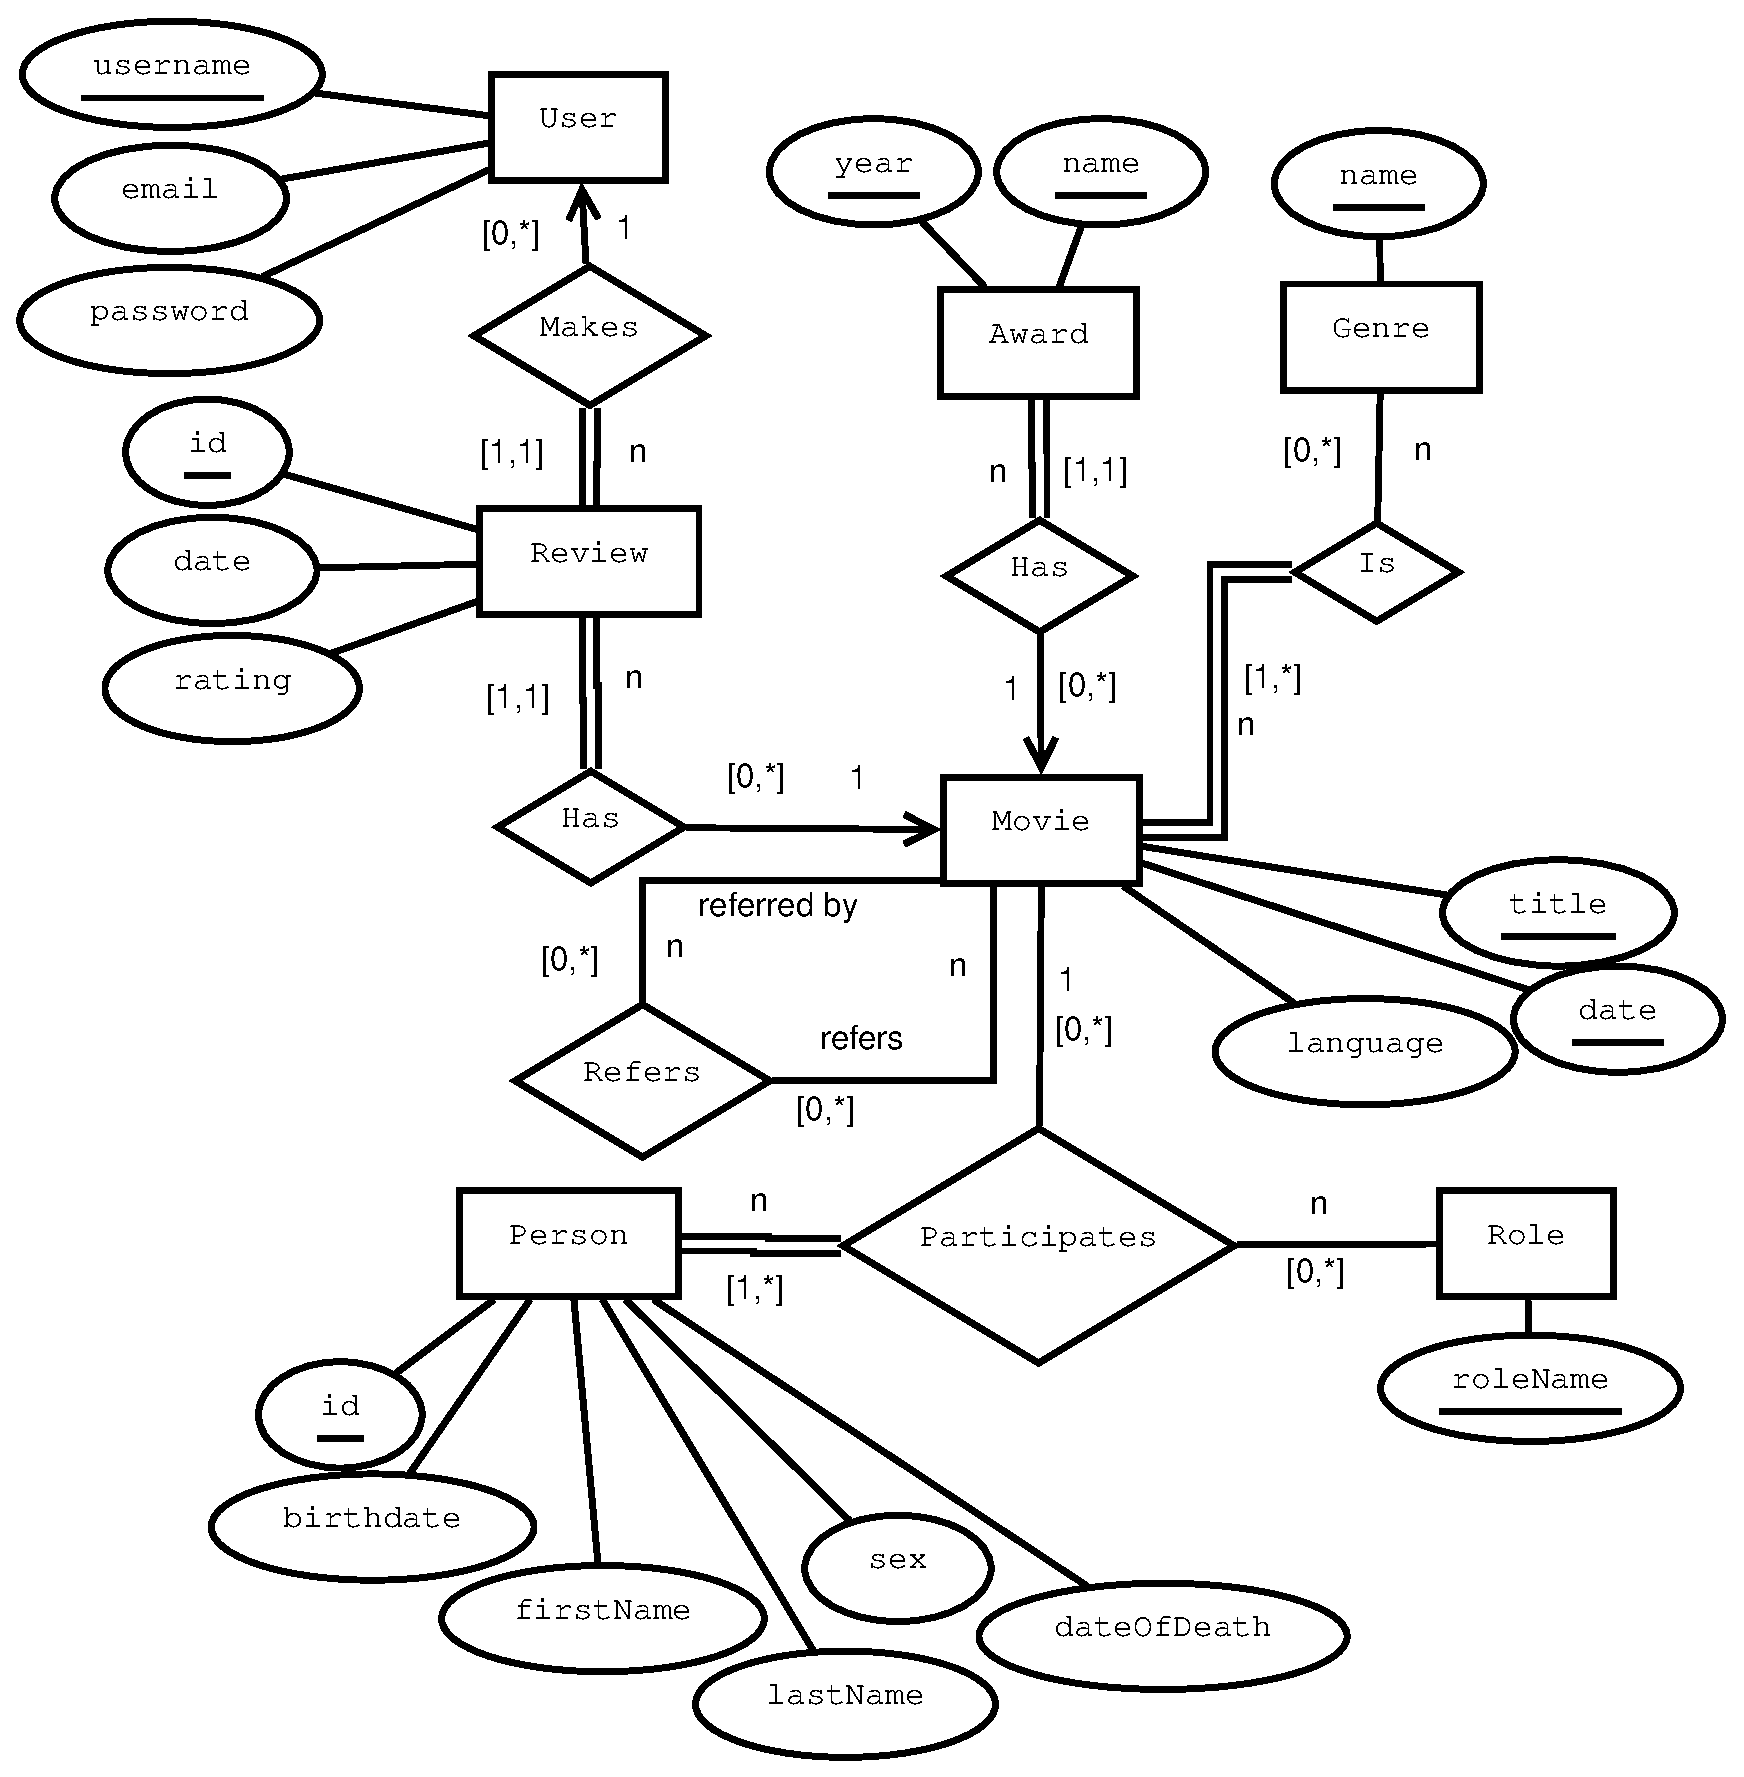
\includegraphics[width=\linewidth]{2-17.02.14/ERDiagram.eps}
  \caption{ER diagram of an IMDB-like website.}\label{fig:ERdiagram2}
\end{figure}

Primary keys are underlined. Chen, min max, and arrows on lines represent the different cardinalities between entities and their relations. Circles are attributes and squares represent entities. Diamonds are relationships, just like we have learned in the course.

\subsection{Schema}
The entities and relationships have been mapped to relations in the below diagram.
\begin{figure}[H]
  \centering
  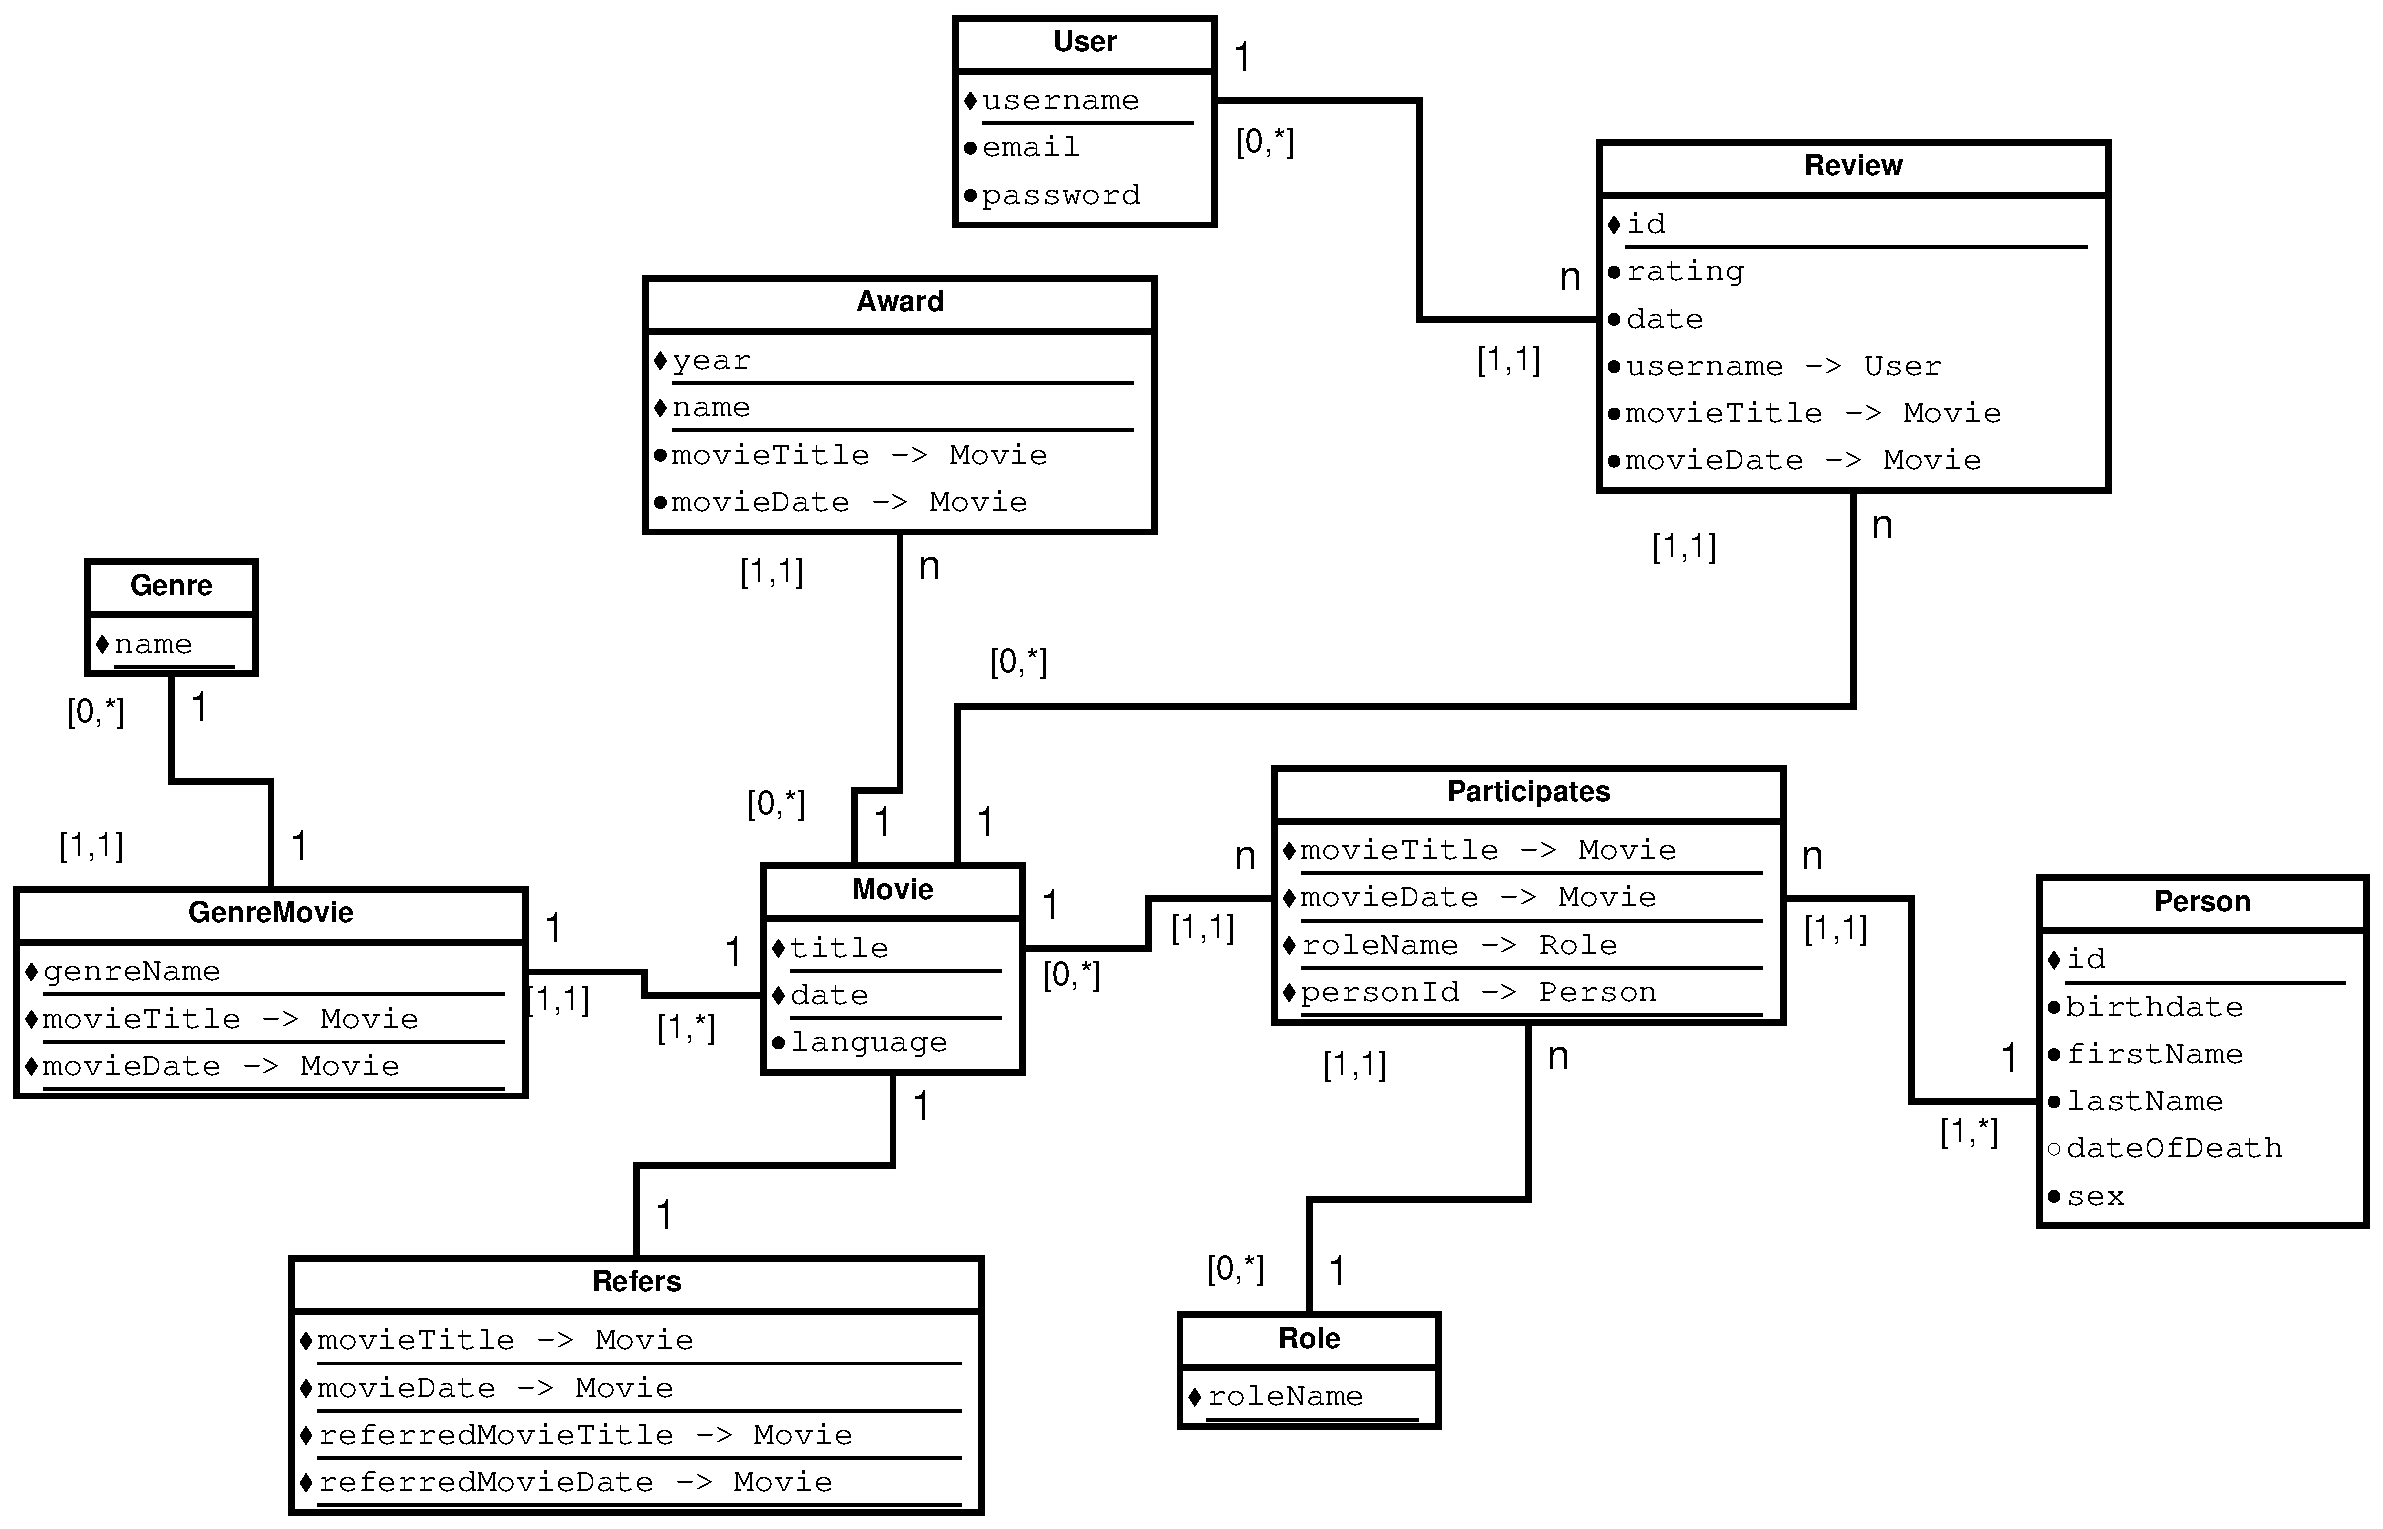
\includegraphics[width=\linewidth]{2-17.02.14/DatabaseSchema.eps}
  \caption{The schema, i.e.\ mapped relations of an IMDB-like website.}\label{fig:schema}
\end{figure}
Attributes acting as foreign keys in relation $A$ are marked by an ASCII arrow \texttt{->}, where the arrow points to the primary key(s) in relation $B$.

\subsection{Non-trivial thoughts}
The \emph{Participate} relationship is 3-way due to the fact that many \emph{People} (actors) can have many different roles in different movies, or even multiple roles in one movie. This relationship construct allows us to express both in the database.
